\documentclass[a4paper,12pt,ngerman]{scrartcl}
\usepackage{babel}
\usepackage{mathptmx}
\usepackage[T1]{fontenc}
\usepackage[utf8x]{inputenc}
\usepackage[a4paper,lmargin=2.5cm,rmargin=2.5cm,tmargin=2.0cm,bmargin=2.0cm,footskip=0.5cm]{geometry}
\usepackage{amsmath}
\usepackage{amssymb}
\usepackage{graphicx}
\usepackage{hyperref}

\hypersetup{
  colorlinks   = true, %Colours links instead of ugly boxes
  urlcolor     = blue, %Colour for external hyperlinks
  linkcolor    = blue, %Colour of internal links
  citecolor    = red %Colour of citations
}

\addtokomafont{sectionentry}{\normalfont}
\addtokomafont{section}{\normalfont}
\addtokomafont{subsection}{\normalfont}

\setcounter{tocdepth}{2}

\graphicspath{ {./images/} }

\renewcommand{\baselinestretch}{1.5} 

\begin{document}
\begin{titlepage}
	Projekttitel: Debuggen mit KI
	\vspace{1cm}
	
	Teilnehmende: PLACEHOLDER
	
	Erarbeitungsort: Zuhause
	
	Projektbetreuende: PLACEHOLDER
	
	Thema des Projekts: Kann eine KI beim Debuggen eines Programms helfen?
	
	Fachgebiet: Informatik
	
	Wettbewerbsparte: Jugend forscht
	
	Bundesland: PLACEHOLDER
	
	Wettbewerbsjahr: 2024
	
	\vspace{2cm}
	\vfill
\end{titlepage}
\clearpage
\tableofcontents
\clearpage

\section{Fachliche Kurzfassung}

Unsere Frage ist es, ob es möglich ist, dass eine KI für einen Programmierer den Debug Prozess übernimmt und selbstständig im Code den Grund für gegebene Fehler finden kann, ähnlich dazu, wie man es als Programmierer tun würde. Hierzu fügen wir eine Middleware in den Debug Prozess von VSCode zwischen Editor und Debug Adapter ein, welcher in der Kommunikation des Debuggers Nachrichten mitlesen, unterbrechen und hinzufügen kann. Eine große Herausforderung ist, wie die KI mit dieser Middleware kommunizieren wird, da LLMs nur Text Nachrichten empfangen und zurücksenden können. Wir benötigen also eine Konvertierung zwischen dem Debug Adapter Protokoll (DAP) und einem für die KI interpretierbaren und produzierbaren Text.

Um den Debug Prozess auf diese Art und Weise verändern zu können, benutzen wir eine VSCode Extension, die beim Starten des Debug Adapters die Funktionen, die zur Kommunikation benutzt werden, mit eigenen Funktionen ersetzt, welche mit der KI kommunizieren und Nachrichten weiterhin mit den originalen Funktionen an den Editor oder an den Debug Adapter senden können.

Nun müssen die Daten des Debug Adapters (DA) in für die KI verständliche Begriffe übersetzt werden. Hierfür stellen wir der KI verschiedene Kommandos zum Empfangen oder Senden zur Verfügung, die von einem Übersetzer in DAP Nachrichten umgewandelt werden. Die KI kann so beispielsweise Breakpoints setzen, das Programm weiterlaufen lassen, oder den Wert einer Variable erfragen. Folgende Kommandos sind für die KI zum Senden verfügbar:
\begin{itemize}
	\item ``BREAKPOINT [Zeile] [Datei]'' (setzen eines Breakpoints)
	\item ``CONTINUE'' (Programm weiterlaufen lassen)
	\item ``STEP'' (Einen Programmschritt ausführen)
	\item ``STEPINTO'' (In einen Funktionsaufruf eintreten)
	\item ``STEPOUT'' (Aus einem Funktionsaufruf austreten)
	\item ``VARIABLE [Name]'' (Variablen auslesen)
	\item ``LINE [Zeile] [Datei]'' (Einzelne Zeilen von Dateien auslesen)
	\item ``ERROR [Fehlermeldung]'' (Wenn die KI, nachdem sie die Anweisungen erhalten hat, irgendetwas vom debuggen abhält)
	\item ``CAUSE [Beschreibung]'' (Wenn schlussendlich der Grund für den Bug gefunden wurde).
\end{itemize}
Außerdem kann die KI folgendes Kommando erhalten:
\begin{itemize}
	\item ``PAUSED [Zeile] [Spalte] [Datei]'' (Wenn das Programm pausiert).
\end{itemize}

Zum Testen dieser KI haben wir sie mit verschiedenen Bugs ausprobiert und jeweils beurteilt, wie hilfreich die Antwort der KI zum Beheben der Bugs war. Hierbei sind wir zum Schluss gekommen, dass die KI mit den gegebenen Kommandos in der Lage ist, erfolgreich Breakpoints zu setzen und anschließend Schrittweise durch ein Program durchzugehen, wodurch es einfache Bugs finden und beschreiben kann. Allerdings ist uns auch aufgefallen, dass die KI mit den gegebenen Kommandos noch Probleme hat komplexere Datenstrukturen im Code nachzuvollziehen.

Aus unseren Ergebnissen schließen wir, dass KIs bereits heute in der Lage sind, den Debug Prozess zu übernehmen und zu steuern, auch wenn sie in unseren Tests noch nicht komplexe Bugs finden konnte. Aus diese Grund sehen wir allerdings in diesem Bereich auch noch viel Potenzial für weitere Entwicklung, um die KI besser als Debugger einsetzen zu können.

Der Code für unser Projekt ist öffentlich auf GitHub verfügbar: \url{https://github.com/Papierkorb2292/AI-Debugger}

\section{Motivation und Fragestellung}

Mit den letzten Fortschritten und dem öffentlichen Zugang zu KI, werden viele Möglichkeiten untersucht, wie eine KI beim Programmieren helfen kann. So gibt es beispielsweise schon länger die Möglichkeit Code Vorschläge von einer KI wie Tabnine oder Github Copilot zu erhalten und mit LLMs, wie ChatGPT, lässt sich auch ein ganzer Codeblock automatisch schreiben.

Wir haben uns gefragt, ob KI Programmierenden auch beim Debuggen von geschriebenen Programmen helfen kann. Die KI ``Devin'' kann bereits selbst Programme schreiben und debuggen, benutzt allerdings zum debuggen \texttt{print} Statements, um den Zustand des Programms zu überwachen, indem dieser stellenweise in die Textausgabe geschrieben wird. Unser Ziel ist es jedoch die KI mit einem Debug Server, den auch Programmierende in ihrem Editor sonst benutzen, kommunizieren zu lassen. Ein weiterer Vorteil hiervon ist, dass es möglich wäre selbst zusammen mit der KI zu debuggen, indem man die KI nur Teile des Debuggen übernehmen lässt, und man den Rest noch selbst über den Editor vornimmt.

\section{Hintergrund und theoretische Grundlagen}

\subsection{KI}

Als KI (Künstliche Intelligenz) bezeichnet man häufig Verfahren zur Datenverarbeitung, für die keine genaue Handlungsanweisung festgelegt werden, sondern die mit Hilfe von Maschinellen Lernen erstellt wird, was einfach gesagt bedeutet, dass man die Parameter des Verfahrens stückweise ändert, um bei Eingangsdaten, für die schon Ausgangsdaten bekannt sind, die Ausgangsdaten des Verfahrens so nah wie möglich an die Erwarteten zu bekommen$^1$. Oft liegt der KI ein neuronales Netzwerk zugrunde, in welchem Eingangsdaten über mehrere Iterationen hinweg verschieden gewichtet und addiert werden können, um am Ende auf die Ausgangsdaten zu kommen.

Als LLM (Large Language Model) bezeichnet man KIs, die Textdaten verarbeiten und auf solche trainiert sind$^3$. Ein bekanntes Beispiel ist ChatGPT: Eine KI, welcher der Benutzer Textanfragen schreiben, und die dann selbst eine Textantwort produziert. LLMs zeichnen sich zudem durch ihre Flexibilität aus, da sie viele verschiedene Aufgaben über Text erledigen können und die Möglichkeit haben vielen Fragen zu beantworten$^2$.

\subsection{Debugging}

Beim Debuggen eines Programm mit einem Debugger, verbindet sich der Editor mit einem Debug Server, der das Programm ausführt und das Programm auch pausieren kann, damit der Editor den Zustand des Programms zu einem bestimmten Punkt anzeigen kann. Während das Programm pausiert ist, lässt sich außerdem mit dem Editor Schritt für Schritt durch das Programm durchgehen, um die Änderungen im Zustand des Programms zu beobachten.

\subsection{Debug Adapter}

Weil ein Debug Server direkt mit dem auszuführenden Programm interagiert, ist die Schnittstelle zum Debug Server oft spezifisch zur Sprache des Programms. Um den Editor mit dem Debug Server zu verbinden, wird deshalb ein Debug Server Adapter benutzt, der spezifisch zu einem Debug Server ist, und für welchen die Kommunikation mit dem Editor von Microsoft auf das Debug Adapter Protokoll (DAP) festgelegt wurde. Für jeden Debug Server kann so auch ein Debug Adapter angeboten werden, der mit dem Debug Server kommunizieren kann$^4$.

Folgendes ist eine Veranschaulichung, wie der Debug Prozess also aufgebaut ist:

\begin{center}
	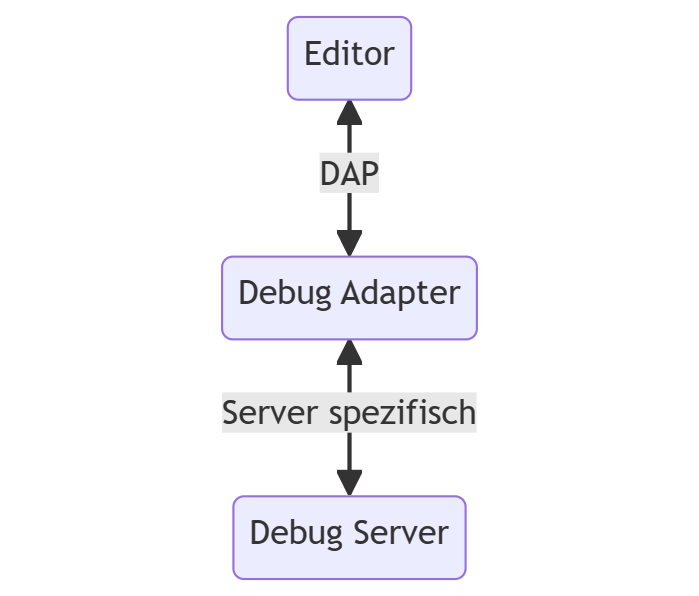
\includegraphics[width=0.5\textwidth]{debugger}
\end{center}

\section{Vorgehensweise, Materialien und Methoden}

Um zu testen, ob es möglich ist, eine KI auf diese Art und Weise beim Debuggen unterstützen zu lassen, werden wir selbst unsere Idee hierzu umsetzen, und verschiedene Ansätze, um mit der KI zu interagieren, auszuprobieren.

Um eine KI in den Debug Prozess zu interagieren, fügen wir zunächst eine Middleware zwischen Editor und Debug Adapter hinzu, durch welche alle Nachrichten zwischen dem Editor und Debug Adapter laufen, damit die KI diese beobachten und unterbrechen kann. Außerdem wird es hiermit möglich, Nachrichten, die durch die KI eingebracht werden, an den Editor und Debug Adapter zu senden. Dies macht es möglich für die KI, Kontrolle über den Debug Prozess zu nehmen.

Es gibt verschiedene Möglichkeiten, wie die KI selbst laufen kann. Zunächst werden wir von OpenAI das KI Modell GPT-4o benutzen, mit welchem man über das Internet kommuniziert. Es wäre außerdem möglich später verschiedene KI Modelle auszuprobieren, um zu testen, wie gut verschiedene Modelle debuggen können.

\subsection{KI Debugger Dienst}

Der wichtigste Teil ist allerdings, wie die KI mit ihren Nachrichten mit dem Benutzer, dem Editor und dem Debug Adapter kommuniziert. Der Benutzer muss nämlich die Möglichkeiten haben, Nachrichten an die KI zu senden, die KI muss antworten können, und zusätzlich muss eine Übersetzung zwischen DAP Nachrichten (normalerweise werden diese zwischen Editor und Debug Adapter gesendet) und dem Text, über welchen die KI kommuniziert, stattfinden. Im folgenden wird dieser Teil als ``KI Debugger Dienst'' betitelt. Außerdem muss der Editor den Kontext, also beispielsweise den Inhalt der Dateien, in denen gedebuggt wird, an den KI Debugger Dienst senden, damit dieser weiß, welche Positionen in den Dateien den verschiedenen Teilen des laufenden Programms entsprechen, um an diesen Stellen pausieren zu können und den Kontext einer Pause zu verstehen.

Folgendes Diagramm veranschaulicht den nun erweiterten Aufbau des Debuggers zusammen mit der Kommunikation mit der KI.

\begin{center}	
	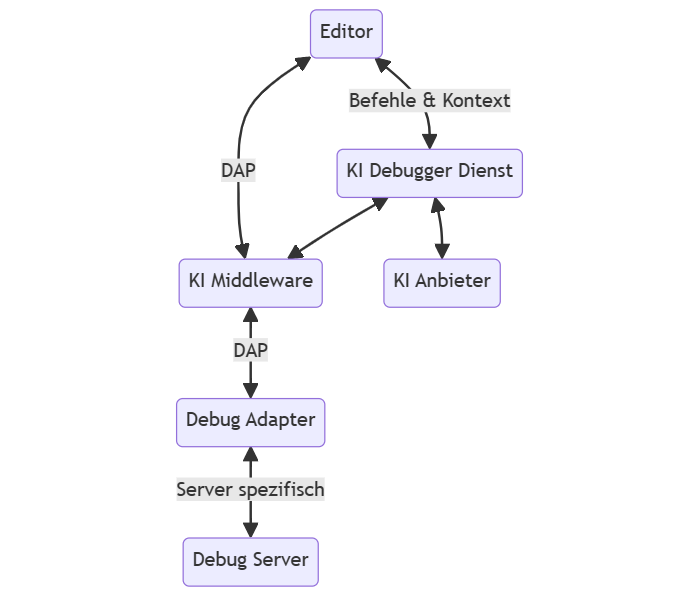
\includegraphics[width=0.5\textwidth]{ai_integration}
\end{center}

Um zu verstehen, wie die Kommunikation zwischen dem Debug Adapter und dem KI-Debugger-Dienst funktioniert, betrachten wir erstmal genauer, wie der KI-Debugger-Dienst die verschiedenen Nachrichten verarbeitet:

Da DAP Nachrichten im JSON Format gesendet werden und dabei oft viele Informationen über den Zustand des Programms enthalten, bei denen wichtig ist, dass sie akkurat sind, wie Dateipfade, Breakpoint Ids, etc., haben wir uns dagegen entschieden, die KI direkt diese JSON Objekte lesen und auslesen zu lassen, da dann die KI viel mehr Wert darauf legen müsste, vollständig fehlerfreie JSON Objekte auszugeben, was die Qualität des eigentlichen Debuggens beinträchtigen könnte.

Stattdessen kommuniziert die KI mit dem KI Debugger Dienst über simple Textnachrichten, von denen jede ein Kommando darstellt. So ein Kommando ist aufgebaut aus einem Kommando Namen und einer Liste von Argumenten, die das Kommando benötigt. Beispielsweise gibt es das Kommando ``BREAKPOINT [Zeile] [Datei]'', welches der KI erlaubt einen Breakpoint in einer bestimmten Datei und Zeile zu setzen, was bedeutet, dass das Programm pausiert, wenn es diese Zeile erreicht. Über die gleiche Art und Weise werden auch bestimmte Events der KI mitgeteilt, indem die KI beispielsweise das Kommando ``PAUSED [Zeile] [Spalte] [Datei]'' erhält, sobald das Programm pausiert.

Alle der KI zur Verfügung stehenden Kommandos werden ihr in der ersten Nachricht mitgeteilt, zusammen mit ihrem Sinn als Debugger und dem zu behebenden Bug. Das Vermitteln der Kommandos geschieht hierbei durch festgelegte Sätze, diese Kommandos werden also in eine sprachliche Form gebracht, die die Kommunikation mit dem LLM ermöglicht. Beispielsweise entspricht das Kommando ``BREAKPOINT'' dem Satz: ``You can set breakpoints in the code by starting your message with "BREAKPOINT" followed by the line number and the file name.'' Dieses Prinzip wird auf jedes Kommando angewendet. Nun, da die Befehle für die KI vorliegen, werden diese übermittelt und die Antworten empfangen. Die jeweiligen Antworten sind so formatiert, dass sie ohne großen Aufwand weiterverarbeitet werden können.

Da wir davon ausgehen, dass die KI nicht immer die Fragestellung ausreichend verstehen wird, haben wir ihr außerdem die Möglichkeit gegeben, Fehler auszugeben, indem sie das Kommando ``ERROR [Fehlermeldung]'' sendet. Dieses Kommando wird an den Editor weitergeleitet, sodass ein User die Fehlermeldung sehen kann und die Anfrage anpassen kann.

Wie bereits erwähnt ist es außerdem wichtig, dass die KI Zugriff auf den Code des Programs bekommt. Auch hierfür gibt es ein Kommando, welches eine Zeile aus einer Datei zu der KI senden kann, wenn die KI ``LINE [Zeile] [Datei]'' sendet. Hierbei meiden wir, eine gesamte Datei auf einmal an die KI zu senden, da dies darfür sorgen könnte, dass die KI sich nicht den genauen Inhalt der einzelnen Zeilen richtig merken kann. Außerdem würde, wenn man der KI eine ganze Datei senden würde, dies viele Tokens verbrauchen, was schlussendlich dafür sorgen würde, dass der Debug Prozess mehr Geld köste.

\subsection{Einbinden der KI}

Dieses Kommando System muss nun in den Debug Prozess eingebunden werden, da im Moment noch das Erhalten und Senden von Kommandos unabhängig vom Debuggen passiert. Hierfür haben wir der KI zusätzlich folgende Kommandos zur Verfügung gestellt, mit Hilfe derer sie ähnlich wie der User mit dem Debug Prozess interagieren kann: ``CONTINUE'', ``STEP'', ``STEPINTO'', ``STEPOUT''. Jeder dieser Kommandos entspricht einem Knopf im Editor, den der Benutzer drücken kann, um das Programm weiterlaufen zu lassen, oder um Schritt für Schritt durch das Programm zu gehen. Wenn die KI ein solches Kommando sendet, wird eine entsprechende DAP Nachricht an den Debug Adapter gesendet, während außerdem eine Nachricht an den Editor gesendet wird, die diesem sagt, der Debug Adapter wäre von alleine weitergelaufen, sodass der User den Verlauf des Debuggens gut mitverfolgen kann.

Während in Folge eines dieser Kommandos das Program weiterläuft, bis es am nächsten Breakpoint angekommen ist oder den angeforderten Schritt ausgeführt hat, wird hingegen die Konversation mit der KI pausiert. Diese geht erst weiter, wenn das Programm wieder pausiert hat, woraufhin die bereits genannte ``PAUSED'' Nachricht an die KI gesendet wird. Auf diese Art und Weise erhalten wir eine Art Rückkopplung, die abwechselnd den Debug Prozess oder die KI laufen lässt und so der KI das schritthafte Debuggen ermöglicht.

Ein zusätzliches wichtiges Kommando ist ``VARIABLE [Name]'', welches der KI erlaubt den Wert einer Variable zu erfragen, sodass die KI den Zustand des Programms aktiv verfolgen kann und dadurch direkt Rückschlüsse darauf ziehen kann, an welcher Stelle im Code der Zustand vom erwarteten Zustand abweicht.

Zuletzt hat die KI außerdem ein ``CAUSE [Beschreibung]'' Kommando, mit dem sie zum Abschluss den von ihr herausgefunden Grund ausgeben kann, warum der Bug aufgetreten ist.

\subsection{Komprimierung der Konversation}

Ein weiterer wichtiger Aspekt ist die Komprimierung der übermittelten Daten. Dies ist aufgrund des Bezahlmodells von OpenAI wichtig, das nach dem Prinzip sogenannter 'Tokens' fungiert, für deren Anzahl man bezahlt$^7$. Dieser Prozess heißt Tokenisierung und funktioniert nach Folgender Reihenfolge:
\begin{enumerate}
	\item Normalisierung des Textes: Im Kern wird hier nichts weiter gemacht als Großbuchstaben in Kleinbuchstaben umgewandelt und unnötige Leerzeichen entfernt werden.
	\item Aufteilung: Der normalisierte Text wird nun in Wörter zerlegt. Dies kann durch das Aufteilen an Leerzeichen und Satzzeichen geschehen.
	\item Tokenisierung: Der nun vorliegende Text wird zum Schluss von Algorithmen zerlegt und in Tokens mit einer vordefinierten ID eingeteilt. Aufgrund dieser ID ist es dem GPT Modell möglich das Wort zu interpretieren.
\end{enumerate}

Beispielsweise wird der Satz ``Die Abkürzung für Künstliche Intelligenz ist KI'' in folgende 16 Tokens aufgeteilt$^10$:\\
\texttt{Die| Ab|k|ür|zung| für| K|ünst|liche| Int|ell|igen|z| ist| K|I}

Unser Ziel ist also so viel sogenannte 'one-word-tokens' zu verwenden wie möglich. Um das zu erreichen, benutzen wir KI, speziell das ChatGPT-4o Modell, um Prompts zu optimieren.

\subsection{Erheben von Daten}

Da nun die KI in den Debug Prozess integriert wurde, ist der nächste Schritt die Fähigkeiten der KI auszutesten, um herauszufinden, ob sie tatsächlich in der Lage ist, ein Programm erfolgreich zu debuggen. Hierfür haben wir uns entschieden, die KI auf verschiedene Probleme zu testen, die wir selbst in Programmen eingebaut haben, und die KI dabei zu beobachten, wie sie diese Probleme löst.

Hierbei können wir für jedes Problem beurteilen, wie präzise und für den User verständlich sowie hilfreich die KI den Grund für das Problem formulieren kann. Außerdem können wir beurteilen, wie sehr sie es geschafft hat den zugrundeliegenden Fehler zu erkennen, oder ob es ihr auschließlich gelang einen Folgefehler zu erkennen. Um dies zu tun, haben wir insgesamt sieben Funktionen geschrieben, von denen jede einen Bug mit steigender Komplexität enthält, den die KI gefragt wird zu finden.

\section{Ergebnisse}

Alle Test Funktionen und die Ergebnisse der KI sind unter folgendem Link zu finden: \url{https://github.com/Papierkorb2292/AI-Debugger/blob/c08f8f01a267f1b80094e715a3c8b819b1061ae7/testWorkspace/test.py}

Bei den ersten Tests hatte die KI zunächst Probleme zu verstehen, dass sie überhaupt Debuggen soll, und meinte unter anderem, dass es ihr schlichtweg nicht möglich wäre Code zu debuggen, obwohl der KI die Kommandos bereitgestellt wurden. Nachdem wir die erste Prompt angepasst haben, konnte die KI die Kommandos korrekt erkennen und erfolgreich den Debug Prozess übernehmen.

Folgendes sind die Ergebnisse der KI für die verschiedenen Funktionen:

\begin{itemize}
	\item Funktion 1 (Fakultät wird mit Addition statt Multiplikation berechnet): Die KI konnte den Bug finden und korrekt beschreiben
	\item Funktion 2 (Bei der Summenberechnung wird mit Index 1 statt 0 angefangen): Die KI konnte den Bug finden und korrekt beschreiben
	\item Funktion 3 (Bei der Maximumfindung wird der \texttt{<} statt dem \texttt{>} Operator verwendet): Die KI konnte den Bug finden und korrekt beschreiben
	\item Funktion 4 (Bei der Primzahlbedingung fehlt bei Quadratzahlen der zweithöchste Teiler): Die KI konnte den Bug finden und eine mögliche Behebung beschreiben, hat aber nicht direkt die Verbindung zu Quadratzahlen gezogen, sondern den Bug stattdessen als ein generelles Problem beschrieben, ohne auf spezifischen Input einzugehen.
	\item Funktion 5 (Bei der Bestimmung, ob die Position in dem Intervall liegt, wird das Ende nicht als Exklusiv, sondern Inklusiv betrachtet): Die KI konnte den Bug finden und korrekt beschreiben
	\item Funktion 6 (Wenn \texttt{tree is None} zutrifft, sollte eigentlich -1 statt 0 zurückgegeben werden): Die KI erkennt zwar, dass bei Leaf Nodes nicht der richtige Wert zurückgegeben wird, allerdings denkt die KI, dass dies gelöst werden kann, indem man \texttt{return 1} mit \texttt{return 0} ersetzt, obwohl im Code bereits \texttt{return 0} an der entsprechenden Stelle steht, was eigentlich mit \texttt{return -1} ersetzt werden muss. Es sind hier also nur Ansätze der richtigen Lösung vorhanden.
	\item Funktion 7 (Bei der Implementation des Algorithmus wurde vergessen, rekursiv für die Child Nodes zu überprüfen, ob sie balanziert sind): Die KI meint fälschlicherweise, dass der Fehler im Algorithmus für Höhe läge, denn obwohl der Bug dort behoben wurde, schlägt sie wieder vor \texttt{return 1} mit \texttt{return 0} zu ersetzen (Obwohl im Code \texttt{return -1} stand).
\end{itemize}

Während wir die Tests durchgeführt haben, ist uns aufgefallen, dass die KI oft dazu neigt, sich,verglichen zum normalen Debuggen, nicht genug über den Code und den Zustand des Programms zu informieren. Wenn wir beispielsweise die KI auf eine der Test-Zeilen verwiesen haben (wie \texttt{assert calculate\_factorial(1) == 1}), hat sie sich oft nicht selbst diese Zeile angeschaut, sondern hat direkt blind ein ``STEPINTO'' Kommando ausgeführt. Außerdem hat sie sich dementsprechend auch nicht die Zeilen von vor und nach dem Bug angeschaut, von der sie beispielsweise auf den Aufbau der Binären Bäume hätte schließen können.

\section{Ergebnissdiskussion}

Die Ergebnisse sind vielversprechend, da sie zeigen, dass es heutigen KIs bereits möglich ist die Funktionsweise von Debug Prozessen zu verstehen und zu reproduzieren.

Allerdings muss auch beachtet werden, dass die Bugs in unseren Tests für die KI speziell für dieses Projekt eingebaut wurden, und es somit eine Abweichung von natürlich auftretenden Bugs geben könnte. Außerdem waren die Algorithmen, in denen wir diese Bugs eingebaut haben, häufig vorkommende Algorithmen, bei denen es möglich wäre, dass die KI diese bereits kannte. Aus diesen Gründen könnten die Ergebnisse in einem realen Debug Prozess abweichen.

Darüber hinaus ist uns aufgefallen, dass die KI vor allem bei komplexeren Datenstrukturen, wie dem Binären Baum aus Aufgabe 6 und 7, Probleme hatte, den Zustand dieser Datenstruktur aufzurufen. Dies könnte daran liegen, dass sich die KI oft nicht die Funktionsdeklaration angeschaut hat, da direkt in der ersten Zeile der Funktion pausiert wurde, sodass die KI nicht sicher wusste, wie die Parameter der Funktion heißen. Außerdem ist der Zugang, den die KI zu Variablen hatte, limitierter als der für Programmierende, da die KI sich nur direkt die Werte von Variablen ausgeben lassen kann (was bei Funktionen und Objekten häufig nur Speicheraddressen sind), wohingegen Programmierende sich auch den Inhalt dieses Speichers anschauen können. Eine mögliche Lösung hierfür wäre es, der KI auch über die Felder von Objekten zu informieren, sodass sie sich anschließend auch den Inhalt dieser Felder anschauen kann.

Zusätzlich dazu ist das Problem aufgekommen, dass die KI zu wenig Zeilen einliest. Dies ist bestehen geblieben, obwohl wir nach den ersten Tests sie für jeden weiteren Durchlauf in der ersten Prompt nochmal darauf hingewiesen haben, dass sie für Zeilen, deren Code sie nicht weiß, diesen anfordern soll. Weitere Anpassungen der Prompts scheinen nötig zu sein, um die KI dazu zu bringen, genügen Code anzufordern, um den Kontext des Programms verstehen zu können.

\section{Fazit und Ausblick}

\subsection{Fazit}

Zusammengefasst lässt sich sagen, dass wir mit unserem System erfolgreich eine KI in den Debug Prozess zu integrieren konnten, und dass diese KI in der Lage ist, den Debug Prozess zu kontrollieren. In einer solchen Integration sehen wir viele Entwicklungsmöglichkeitein, um einen KI Debugger als ein für Programmierende nützliches Tool bereitzustellen. Wir sind zum Schluss gekommen, dass, auch wenn im Verlaufe der Tests noch weitere Herausforderungen offentsichtlich geworden sind, die KI mit verbesserten Prompts und mehr Kommandos für noch mehr Kontrolle über den Debug Prozess auch kompliziertere Bugs finden könnte, da es bereits andere KIs, wie Github Copilot gibt, die ein großes Verständnis von Programmen aufzeigen und dadurch bereits für Programmierende ein nützliches Tool sind. Würde eine KI mit einem solchen Ausmaß an Verständis von einer Codebase (also einem gesamten Projekt) ebenfalls die Möglichkeit gegeben werden, einen Debug Prozess zu steuern, erwarten wir eine beträchtliche Verbesserung in der Leistung des KI Debuggers.

\subsection{Ausblick}

Zunächst möchten wir darauf aufmerksam machen, dass realistischere Tests zur genaueren Evaluierung der Fähigkeiten der KI notwendig sind, da wir sie nur gegen Bugs getestet haben, die wir selbst eingebaut haben. Hierfür wäre es entweder möglich bei einer Gruppe von Programmierenden über einen längeren Zeitraum Bugs zu sammeln, auf welche dann die Debugger KI getestet werden kann, oder über öffentliche Code Repositories, wie Github, Bugs zu sammeln, da es dort meist eine Liste von gefundenen Fehlern gibt, mit denen die KI getestet werden könnte.

Wir erwarten außerdem, dass sich wesentlich bessere Ergebnisse erzielen lassen würden, wenn man anstatt einer allgemeinen KI, die auf viele verschiedene Aufgaben trainiert ist, eine spezifische KI für das Debuggen trainiert. Es wäre beispielsweise möglich, diese KI auch auf die Syntax von Programmiersprachen spezialisiert zu trainieren, sodass sie das Program und die Aufgabe besser versteht. Ein möglicher Start hierfür wäre die KI Codex von OpenAI, die speziell auf das Verständis von Code trainiert ist. Dies ist auch das KI Modell, auf welchem Github Copilot aufbaut.

Um zusätzliche Trainingsdaten für eine solche KI zu erheben, wäre es möglich die Middleware bei normalen Debug Prozessen mitlaufen zu lassen, sodass die Kommunikation zwischen Editor und Debug Adapter aufgezeichnet wird. Das würde es erlauben die KI auf die aufgezeichneten Daten zu trainieren, sodass sie lernt den Editor und daher auch die Programmierenden nachzustellen. Fraglich ist, ob es möglich wäre von den aufgezeichneten Daten auf das Problem und die Problemlösung zu schließen, oder ob es notwendig wäre, dass die Programmierenden, wenn sie ihre Debug Prozesse aufzeichnen möchten, auch zusätzliche Informationen über das Problem und die anschließend angewandte Lösung angeben müssten, sodass die KI lernen würde das Problem einzulesen und die Lösung auszugeben.

Eine weitere große Verbesserungsmöglichkeit ist es, dem bereits von uns erstelltem System mehr Kommandos hinzuzufügen. Beispielweise könnte man es der KI möglich machen, eine Liste aller Variablen zu erhalten, den Call stack auszulesen (also die Reihenfolge der Funktionsaufrufe zu erhalten) oder auch die Möglichkeit geben, den Wert einer Variable zu ändern. Dies sind Aktionen, die auch beim normalen Debuggen oft nützlich sind, und die es der KI ermöglichen würden, das Programm besser zu debuggen, falls sie ausreichend Codeverständis aufzeigt.

\section{Quellen- und Literaturverzeichnis}

$^1$ Wikimedia Foundation Inc.,  ``Künstliche Intelligenz - Wikipedia'', grundlegende Information zu künstlicher Intelligenz\\
\url{https://de.wikipedia.org/wiki/K\%C3\%BCnstliche_Intelligenz}, besucht am 19.03.2024\\
$^2$ Wikimedia Foundation Inc.,  ``Large language model - Wikipedia'', grundlegende Information zu Large Language Models\\
\url{https://en.wikipedia.org/wiki/Large_language_model}, besucht am 19.03.2024\\
$^3$ Wikimedia Foundation Inc.,  ``Language model - Wikipedia'', grundlegende Information zu Language Models \\
\url{https://en.wikipedia.org/wiki/Language_model}, besucht am 19.03.2024\\
$^4$ Microsoft, ``Overview [über das Debug Adapter Protokol]'', grundlegende Information zum Debug Adapter Protokoll
\url{https://microsoft.github.io/debug-adapter-protocol/overview.html}, besucht am 25.03.2024\\
\vspace{1em}\\
$^5$ Microsoft, ``Extension API | Visual Studio Code Extension API'', Anleitung zum Entwickeln einer VSCode Extension\\
\url{https://code.visualstudio.com/api}, besucht am 19.03.2024\\
$^6$ Microsoft, ``vscode/blob/main/src/vs/workbench/contrib/debug/node/debugAdapter.ts at main microsoft/vscode'', VSCode Quellcode zur Kommunikation mit Debug Adaptern\\
\url{https://github.com/microsoft/vscode/blob/main/src/vs/workbench/contrib/debug/node/debugAdapter.ts}, besucht am 19.03.2024\\
$^7$ OpenAi, ``Introduction - OpenAI API'', Grundlegene Information zum Benutzen der KIs von OpenAPI\\
\url {https://platform.openai.com/docs/introduction}, besucht am 01.07.2024\\
$^8$ OpenAi, ``OpenAI Platform'', Information über\\
\url {https://platform.openai.com/organization/api-keys}, besucht am 01.07.2024\\
$^9$ OpenAi, ``ChatGPT'', Die ChatGPT KI\\
\url {https://chatgpt.com}, besucht am 01.07.2024\\
$^{10}$ OpenAi, ``Introduction - OpenAI API'', Tool zum Ausprobieren, in was für Tokens ein Text von OpenAI aufgeteilt wird\\
\url {https://platform.openai.com/tokenizer}, besucht am 01.07.2024

\end{document}